Machine learning (ML) models may inform real-world decisions with high-stakes consequences. Examples include 
%``Which ICU patients need extra intervention?,'' 
``Is air quality sufficient to go outside now?''~\citep{berlinghieri2026hourly},
``Where should scarce public resources be allocated?''~\citep{heuton2025decisionaware},  or ``Which route should I take?'' \citep{tangPyEPOPyTorchbasedEndtoend2024}. 
Ideally, prediction models would be directly trained to optimize a loss tailored to the stakes of the decisions at hand. When the underlying model is misspecified (as is often the case when dealing with real-world data), this \emph{decision-aware} end-to-end training should make superior decisions~\citep{elmachtoubDissectingImpactModel2025}. 
%For a broader survey of possible end-to-end methods, see~\citet{mandi_decision-focused_2024}.


Many decision problems of practical interest have a loss that is piecewise constant as a function of model parameters. Consequently, gradients of the loss with respect to parameters will be 0 almost everywhere. 
All zero gradients mean that gradient descent, one of ML's go-to tools for parameter learning, will be ineffective. 
%Without informative gradients, an optimizer can never move away from an initial parameter value no matter how bad it is.
To overcome this limitation, many methods have been proposed~\citep{mandi_decision-focused_2024}. 
As the number of methods have increased, new methods papers have appropriately tried to compare their methods to the other options, and a recent benchmark study on so called "Predict-then-Optimize" methods \citep{gengBenchmarkingPtOPnO2024} has attempted to provide a common suite of tasks so that models can be assessed on an equal ground.
%In recent years, several methods papers and benchmark studies have begun to offer apples-to-apples comparisons of different methods on synthetic and real problems. 

% We consider two families of methods here. In Perturbation methods~\citep{abernethyPerturbationTechniquesOnline2016,berthetLearningDifferentiablePerturbed2020}, informative gradients are obtained by adding noise to model outputs.
% The exemplar method we focus on here is the Differentiable Perturbed Optimizer (DPO)~\citep{berthetLearningDifferentiablePerturbed2020}.
% In contrast, Surrogate Loss methods pick another less-flat loss with non-zero gradients instead of the ideal (yet flat) decision loss. Exemplars here include methods known as PG~\citep{huang2024decisionfocusedPG} and SPO+\citep{elmachtoubSmartPredictThen2022}.
% Using their informative gradients, both families estimate parameters via the common toolbox of gradient descent.
% optimization. % to estimate parameters.

%Among the many methods now available, which is recommended for practical use?


%However, we find that Perturbation methods have rarely been featured in such experiments.
%Despite discussing \citeauthor{berthetLearningDifferentiablePerturbed2020}'s DPO in related work, at least two high-profile recent studies~\citep{huang2024decisionfocusedPG,gengBenchmarkingPtOPnO2024} omit DPO entirely from their experiments. 
%Additionally, while the PyEPO benchmark~\citep{tangPyEPOPyTorchbasedEndtoend2024} represents a huge value for the community, unfortunately some released DPO code has a subtle correctness issue (see App.~A).

However, we have found that many of these comparison tasks are not ideal for decision-aware methods. In 6 of the 7 tasks presented in the Predict-then-Optimize benchmark, we show that with a slightly expanded hyperparameter search, the \textit{decision-unaware} approach that trains to minimize prediction error and then later solves the optimization task (called a two-stage approach) is either the best method (4 of 7 tasks) or competitive with the best methods (2 of 7 tasks) as assessed by decision-quality on held out data. \
In fact, if the one task in which the two-stage approach does poorly (Budget Allocation) is excluded, this decision-unaware approach has the highest average rank of all decision-aware methods considered. Fig.~\ref{fig:rank_transition} shows the resulting rank shifts: MSE moves from 5th in the original benchmark to 2nd after the expanded hyperparameter search.
\begin{figure*}[t]
\centering
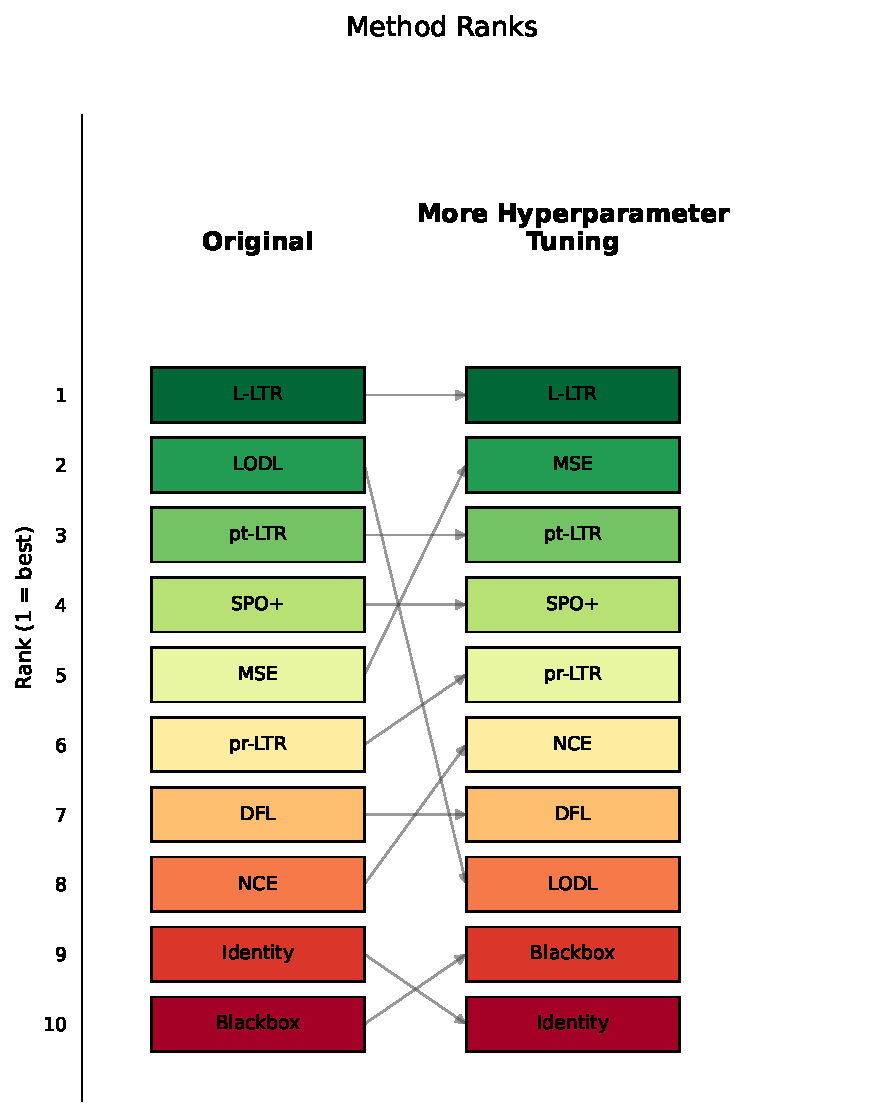
\includegraphics[width=\textwidth]{figures/fig_rank_transition_2col_7tasks.pdf}
\caption[Rank shifts from \citeauthor{gengBenchmarkingPtOPnO2024}'s originally reported results to our hyperparameter-tuned re-run.]{\textbf{Rank shifts from \citeauthor{gengBenchmarkingPtOPnO2024}'s originally reported results (left) to our hyperparameter-tuned re-run (right), averaged across the 7 PnO benchmark tasks.} MSE moves from 5th in the original benchmark to 2nd after the expanded hyperparameter search, illustrating that the decision-unaware baseline was substantially underperforming under the original tuning protocol.}
\label{fig:rank_transition}
\end{figure*}


We attribute this to most benchmark tasks falling into a well-specified regime, where two-stage MSE is known to be advantaged \citep{elmachtoubDissectingImpactModel2025, huFastRatesContextual2022}. \
Following \citet{elmachtoubDissectingImpactModel2025}, we assess the level of misspecification as the gap in decision loss between a two-stage model and a model trained with a decision-aware objective. When this gap is small the task is \emph{well-specified}, and when it is large the task is \emph{misspecified}. This is closely related to the standard statistical notion of misspecification (the model class cannot recover the data-generating $\theta^\star$), but is defined directly in terms of decision quality rather than predictive likelihood.

In this work, we show how several common decision-aware benchmark tasks do not benefit from decision-aware learning. Our contributions are:
\begin{itemize}[leftmargin=*,noitemsep,topsep=0pt]
    \item We re-evaluate end-to-end learning methods from \citeauthor{gengBenchmarkingPtOPnO2024}'s benchmarks (Fig.~\ref{fig:bench_bump}, \ref{fig:budget_bump}, \ref{fig:portfolio_bump}), and show how competitive decision-unaware approaches can be with a slightly expanded hyperparameter tuning grid (more batch sizes and explicit tuning of method-specific parameters not reported in the original benchmark).
    \item We provide an assessment of which tasks are suitable for future decision-aware learning research.
    \item We review the synthetic benchmark task from ~\citet{huang2024decisionfocusedPG} (Fig.~\ref{fig:noisy_synth_sweep},~\ref{fig:noisy_synth_regret}) and contrast it with the Predict-then-Optimize tasks above to make explicit the regime in which decision-aware approaches are truly beneficial.
    \item We revisit the real-world top-K site selection comparison from Chapter~\ref{chap:daml}~\citep{heuton2025decisionaware} (Fig.~\ref{fig:topK_interpolation_main}) and show that what appeared as method-intrinsic differences between decision-aware methods on these tasks largely reflects training-objective alignment with the evaluation metric: surrogate methods reach similar solutions once their per-instance objective is normalized to match the BPR metric.
    %We also examine easy-to-understand synthetic datasets, where we show empirically that DPO shares two desireable properties of best of surrogate loss methods~\citep{huang2024decisionfocusedPG}: (1) DPO's preferred parameter aligns with the ideal regret minimizer even under misspecification; and (2) as training set size increases, estimated model's regret decreases.

    %\item While DPO can work well out of the box, we show several problems where DPO's success is highly sensitive to its noise-level hyperparameter. With improved tuning strategies beyond simple grid search, we find DPO can noticeably improve its regret, though on some tasks no big gains occur.
    
    %\item We further reveal that a strong surrogate method well-suited for misspecified real-world scenarios, PG~\citep{huang2024decisionfocusedPG}, also has a key hyperparameter sensitivity where  even recommended settings can yield subpar regret (see Fig.~\ref{fig:noisy_synth_triptych}).
\end{itemize}
Our work suggests that common benchmarking tasks may be giving an incomplete picture of the relative performance of decision-aware methods, and that too-limited hyperparameter tuning protocols may be obscuring the strength of two-stage, decision-unaware methods (Fig.~\ref{fig:rank_transition}). We hope this spurs greater innovation in benchmarking tasks and deeper understand of the relative strengths and weaknesses in decision-aware learning methods.


%    \item We provide a ``User's Guide'' for key methods from both families tailored to machine learning practitioners. Each guide explains the method's core ideas and inner workings in common notation. Each guide offers clear guidance when a method might be a good fit for the problem at hand, and a clear recipe for hyperparameter tuning backed by reusable code.


%    \item \todo{Update when we know more:} We offer a novel hypothesis for  performance gap of these methods: different loss functions result in different gradient signal to noise ratios. We present preliminary experimental testing of this hypothesis.


% Across both families, all methods considered here share the desirable property that their tractable loss, whether noisy or surrogate, is minimized when the ideal decision loss is minimized. This means that no matter which method is used, good decision-making performance should be obtainable by minimizing its loss. 
% Despite this loss alignment, we observe quite different results for each method empirically in terms of the ultimate decision quality of its estimated parameters. Some performance discrepancy can be explained by varying the degree of model misspecification or the amount and kind of observation noise. However, little attention in the literature has been given to describing the regimes in which each method might be expected to work best. Furthermore, many of these loss functions introduce nuisance hyperparameters, such as the magnitude of the noise in the perturbation methods, or the size of the finite difference gap in the surrogate losses. Correctly tuning these hyperparameters makes all the difference in a model's performance, but there is a dearth of guidance on how to do this.
